\chapter{Results}
\label{Chap4}
Analyses statistiques etc...
\section{Parameters optimisation}

\section{Reproducibility}
\subsection{Relative density and mechanical properties}

\subsection{Melt pool size and distribution}

\section{Internal properties homogeneity}
As said in section \ref{MMFPP}, all tensile specimens were fabricated vertically. Their height is significantly greater than the other samples'; respectively 6 [cm] and 1 [cm] or less. It was chosen to cut up specimen X200-180417-25 into slices to measure if the density and hardness were homogeneous along the Z direction in the material. The surfaces analysed were named according to their original Z position in the specimen with "B", "C1" , "C2", "C3" and "T" (for bottom, center and top) and to the test done with a letter "D" or "H"  (for density and hardness). The denomination is summarised in figure \ref{fig:saus}.\\

\begin{figure}[th]
\centering
\centerline{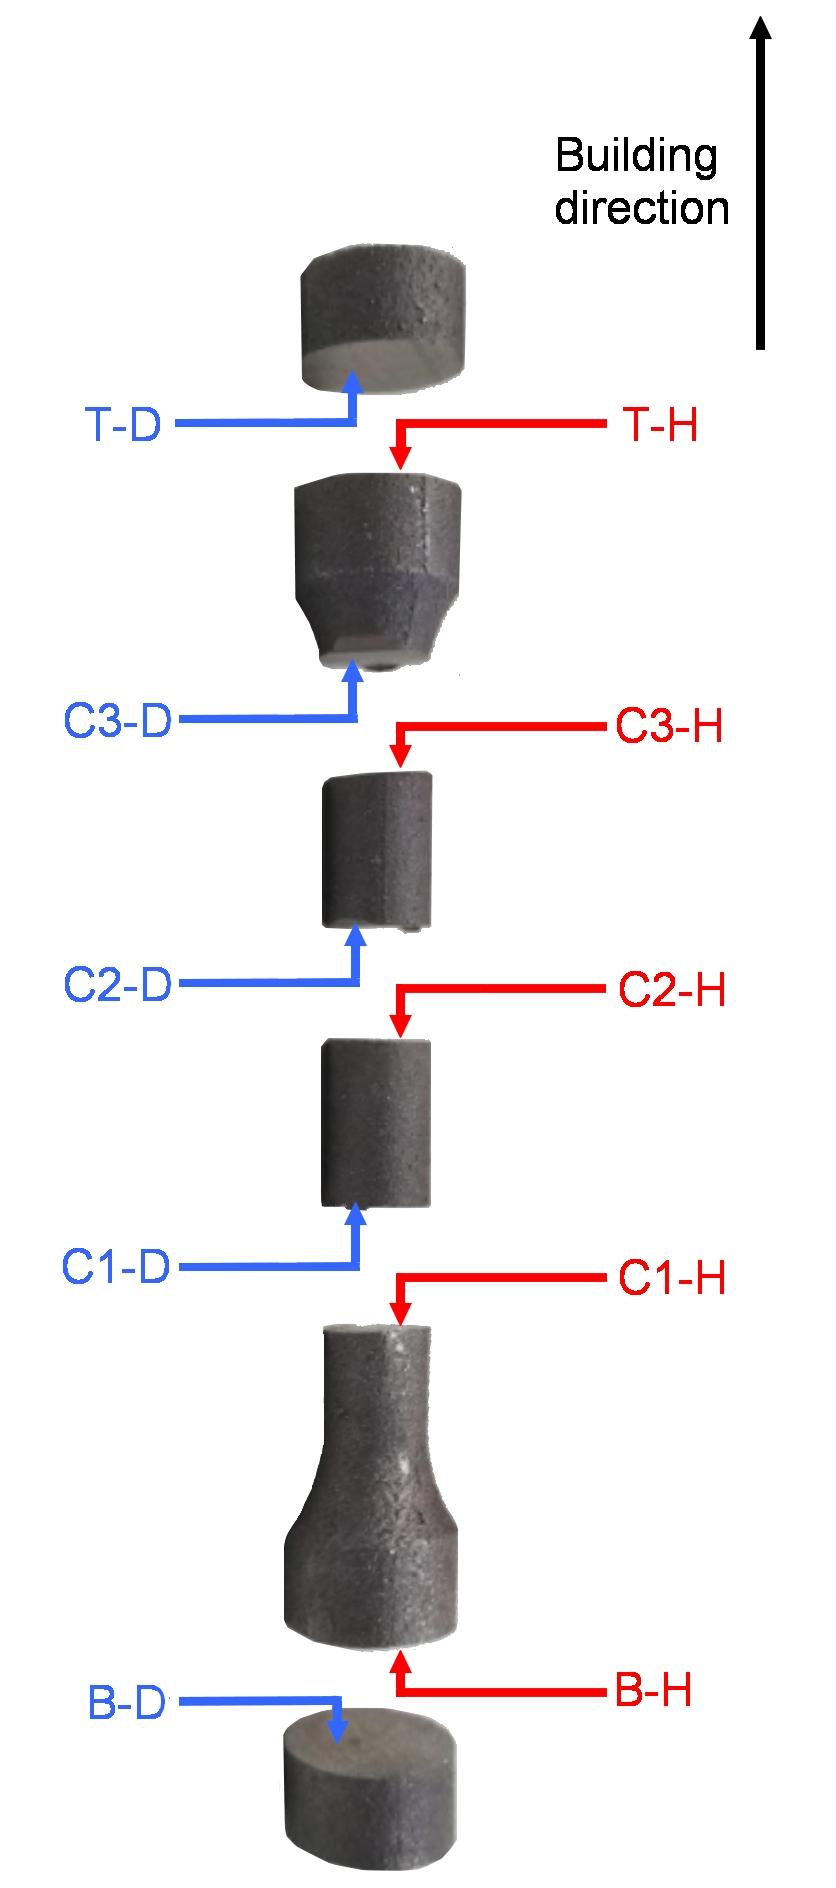
\includegraphics[scale=0.23]{Images/Saus}}
\decoRule
\caption[Specimen X200-180417-25 sub-parts and surfaces denomination]{Specimen X200-180417-25 sub-parts and surfaces denomination.}
\label{fig:saus}
\end{figure}

[Graphe batonnets de H et rho + analyse statistique]

\section{Powder ageing}

\subsection{Grain size and distribution}
\subsubsection{Fresh powder}

\subsubsection{Recycled powder}
\subsection{Composition}

\subsubsection{Fresh powder}

\subsubsection{Recycled powder}
 \begin{center}
\begin{table}[ht]
\begin{tabular}{|c|c |c |c| c|c|}
    \hline
    Date of sampling& Date of last addition of fresh powder & \multicolumn{4}{c}{Composition [\%wt]} \vline\\
    \cline{3-6}
    & & Al& Fe&Mg&Si\\
\hline 
\hline   
    23/10/2017 & 07/09/2017 &89.2&0.12&0.49&10.2\\
    09/01/2018 & 07/09/2017 & 89.3 & 0.13 &0.48&10.1\\
    12/01/2018 & 07/09/2017 & 89.4 & 0.13 &0.48&10\\
    21/02/2018& 07/09/2017 &89.1&0.19&0.51&10.3\\
    13/03/2018& 22/02/2018 &89.1&0.16&0.51&10.1\\    
    \hline
\end{tabular}

\caption[Composition of recycled AlSi10Mg powder as a function of the date]{Composition of recycled AlSi10Mg powder as a function of the date}
\label{tab:compo}
\end{table}
 \end{center}

\section{Heat treatments}

\subsection{Heating process}

\subsection{Microscopy}

\subsection{Hardness testing}

\subsection{Tensile testing}

 \begin{center}
\begin{table}[ht]
\noindent\makebox[\textwidth]{\begin{tabular}{|c|c|c |c |c| c|c|}
    \hline
    Specimen & Contour &  TT & E [GPa] & $\sigma_y$ [MPa] & $\sigma_u$ [MPa] & $\epsilon_f$[\%] \\

\hline
\hline   
    X200-180417-1 & Yes & None & 74.6 & 260.8 & 366.4 & 2.2  \\
    X200-180417-2 & Yes& None & 68.2 & 290.2 & 388.3 & 2.4\\
    X200-180417-3 & Yes& None & 64.0  & 275.9 & - & - \\    
        X200-180417-A& No & None & 61.0 &257.1  & 379.2 & 2.8 \\
    
    X200-180417-7 & Yes& 250$^\circ$C (2h) & 72.2 &230.7 & 334.5 & 9.1 \\
    X200-180417-8 & Yes& 250$^\circ$C (2h) & 70.2 & 238.9 & 347.4 & 8.6 \\
    X200-180417-9 & Yes& 250$^\circ$C (2h) & 71.3 & 227.7 &$\simeq 328.7$ & - \\
    X200-180417-4 & Yes& 300$^\circ$C (2h) & 81.6 & 164.4 & 249.6 & 14.1 \\ 
    X200-180417-5 & Yes& 300$^\circ$C (2h) & 68.4 &172.4 & 256.24 & 13.1 \\
    X200-180417-6 & Yes& 300$^\circ$C (2h) & 68.6 &168.5 & $\simeq 242.5$ & - \\

\hline
\end{tabular}}

\caption[Tensile mechanical properties of the specimens from batch X200-180417]{Tensile mechanical properties of the specimens from batch X200-180417}
\label{tab:pol}
\end{table}
 \end{center}
 
\subsection{Internal stress testing}





%\begin{table}
%\caption{The effects of treatments X and Y on the four groups studied.}
%\label{tab:treatments}
%\centering
%\begin{tabular}{l l l}
%\toprule
%\tabhead{Groups} & \tabhead{Treatment X} & \tabhead{Treatment Y} \\
%\midrule
%1 & 0.2 & 0.8\\
%2 & 0.17 & 0.7\\
%3 & 0.24 & 0.75\\
%4 & 0.68 & 0.3\\
%\bottomrule\\
%\end{tabular}
%\end{table}